% !TEX root = ../main.tex

\section{Project scope}
\subsection{State-of-the-art}
\begin{frame}{\insertsubsec}
  The most typical approach is to extract radiomic features, usually with
  the \emph{PyRadiomics} package, from the MRI, PET or CT scans.

  \vspace{.5cm}
  An alternative approach is to use deep-learning based models for prediction or 
  feature extraction. Pre-trained models have reduced the requirements for big data sets.
  Possible strategies are:
  \begin{itemize}
    \item Use a pre-trained CNN as a feature extractor
    \item Fine tune a pre-trained CNN on medical data
  \end{itemize}
  \vspace{.5cm}
  In survival models \emph{DeepSurv} is uses a deep neural network to fit a Cox Proportional 
  Hazards model
\end{frame}

\begin{frame}
  In 3D imaging \emph{DeepMedic} used 3D CNNs to analyze MRI scans for brain lesion segmentation

  \vspace{.5cm}
  \begin{figure}
    \centering
    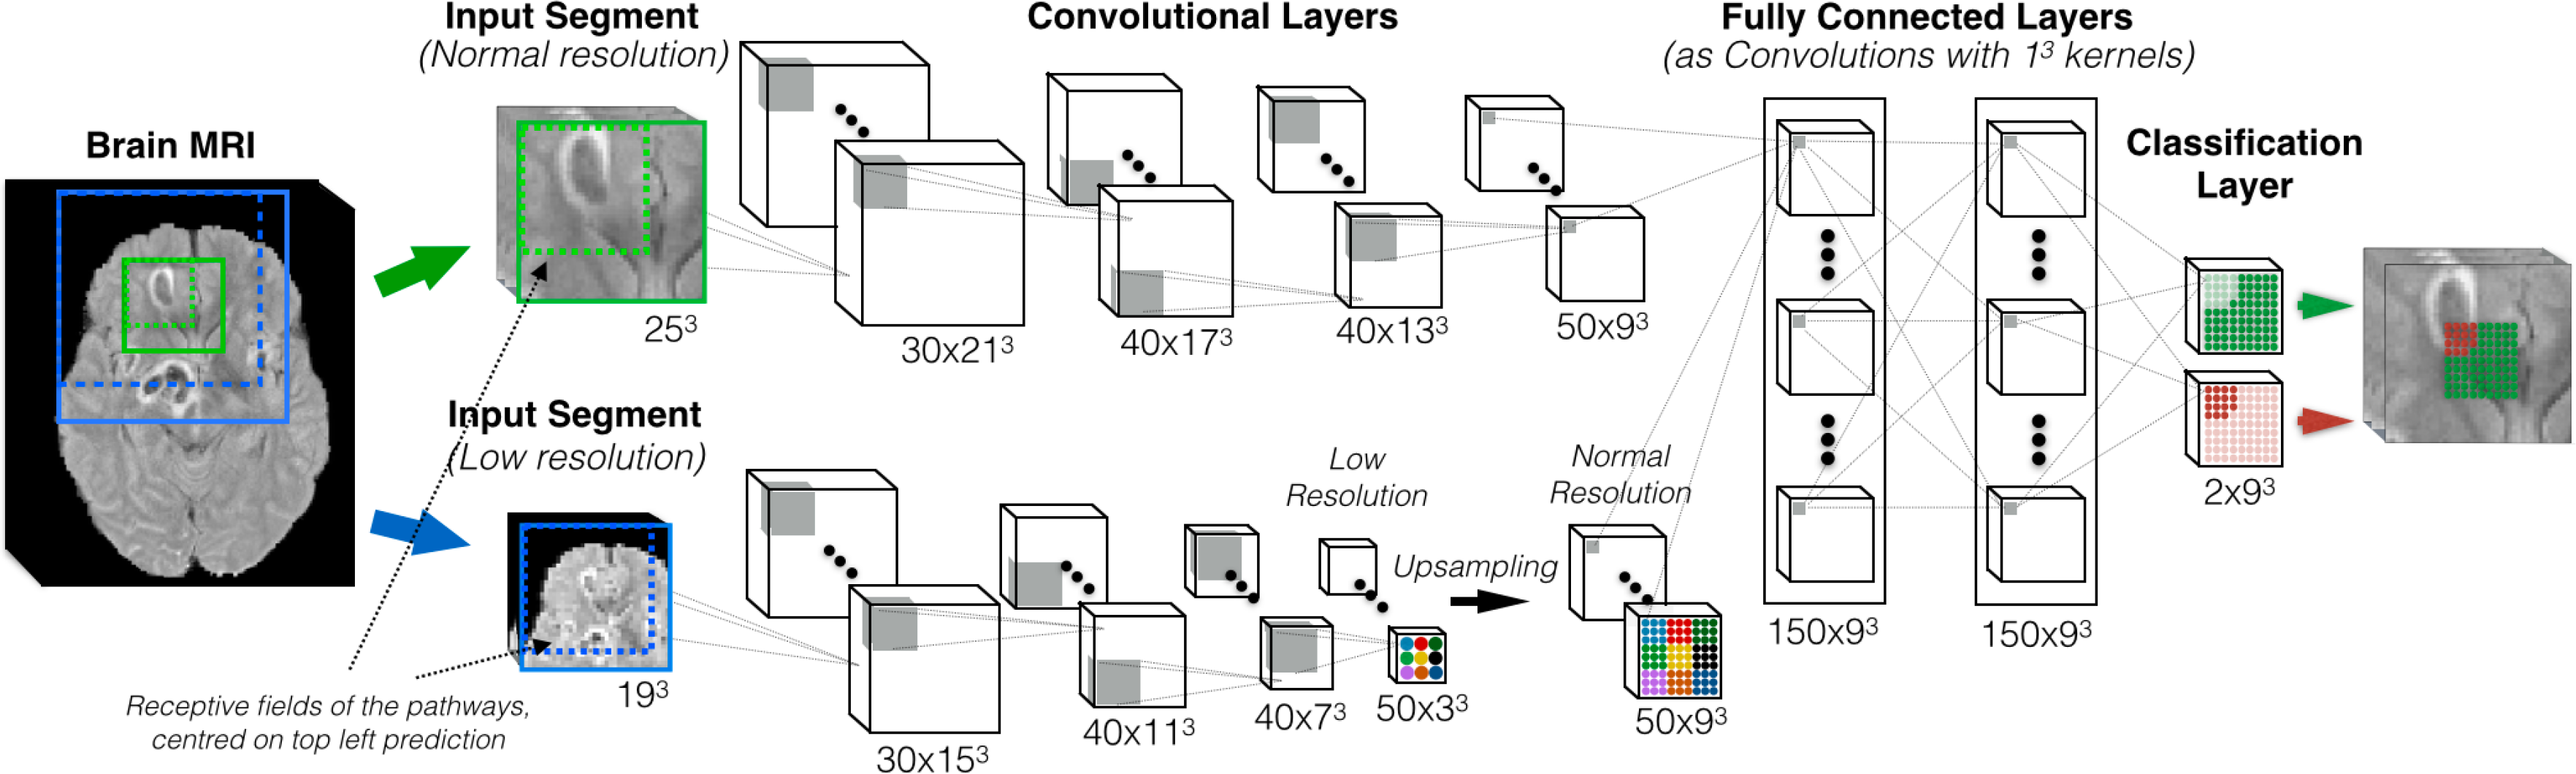
\includegraphics[width=.9\textwidth]{images/deepmedic}
    \caption{\emph{DeepMedic} architecture}
  \end{figure}
\end{frame}

\subsection{Problem formulation}
\begin{frame}{\insertsubsec}

  \begin{itemize}
    \item Work centered around PMHNK dataset
    \item Medical Image analysis problem
    \item Current results show a CI of 0,628
  \end{itemize}
  
  Can a better survival prediction than the current results, be obtained using image
  data and Deep Neural Networks?
\end{frame}

\subsection{Objectives}
\begin{frame}{\insertsubsec}
  \begin{itemize}
    \item Get a better understanding of survival prediction problems.
    \item Be able to analyze the PMHNK dataset to get different strategies for building a 
    deep learning model.
    \item Develop a new deep learning model to improve the survival's prediction rate of
    PMHNK dataset patients.
    \item Investigate and compare the performance of the deep learning-based method to 
    the more conventional methods.
    \item Get a better CI than the \emph{volume} feature, which is often used in clinic as a
    prognostic feature, its CI is 0,628.
  \end{itemize}
\end{frame}

\subsection{Stakeholders}
\begin{frame}{\insertsubsec}
  \begin{itemize}
    \item Developer: responsible for research, document and implement the software
    \item Director: responsible for guiding, giving advice and helping the Developer
    \item Beneficiaries: future researchers or patients depending on the outcome
  \end{itemize}
\end{frame}

\subsection{Methodology}
\begin{frame}{\insertsubsec}
  \begin{itemize}
    \item As a research project it will have a process of trial and error
    \item Once in a while the project will be presented in the lab weekly meetings
    \item Every week a meeting with the Principal Investigator will be scheduled
  \end{itemize}
\end{frame}

\subsection{Obstacles}
\begin{frame}{\insertsubsec}
  Some obstacles may be found during the project:

  \begin{itemize}
    \item Training time
    \item Bugs
    \item Scheduling
    \item Not enough data
  \end{itemize}
\end{frame}
